\documentclass{article}
\usepackage[utf8]{inputenc}

\title{EE2703 A6: The Laplace Transform}
\author{Prasanna Bartakke EE19B106}
\date{\today} % Date for the report


\usepackage{natbib}
\usepackage{graphicx}
\usepackage{amsmath}
\usepackage{listings}

\begin{document}

\maketitle

\section{Introduction}
In this assignment, we will look at how to analyze “Linear Time-invariant Systems” using the scipy.signal library in Python .We limit our analysis to systems with rational polynomial transfer functions. More specifically we consider 3 systems: A forced oscillatory system, A coupled system of Differential Equations and an RLC low pass filter  

\section{Assignment Questions}
\subsection{Time response of a spring system}
Consider the forced oscillatory system given by the equation(with 0 initial conditions):
\begin{equation}
    \ddot x + 2.25x = f(t)
\end{equation}
where
\begin{equation}
    f(t) = cos(1.5t)e^{-0.5t}*u(t)
\end{equation}
Solving for $X(s)$ in Laplace domain we get,
\begin{equation}
    X(s) = \frac{s+0.5}{(s+0.5^2)+2.25)(s^2+2.25)}
\end{equation}
Use the impulse response of $X(s)$ to get its inverse Laplace transform.

\begin{figure}[h!]
\centering
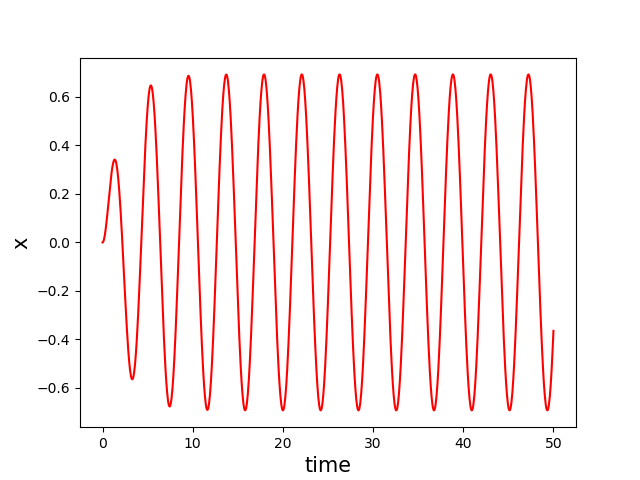
\includegraphics[scale=0.6]{fig0.png}
\caption{System Response with Decay = 0.5}
\label{fig:System Response with Decay = 0.5}
\end{figure}

\begin{figure}[h!]
\centering
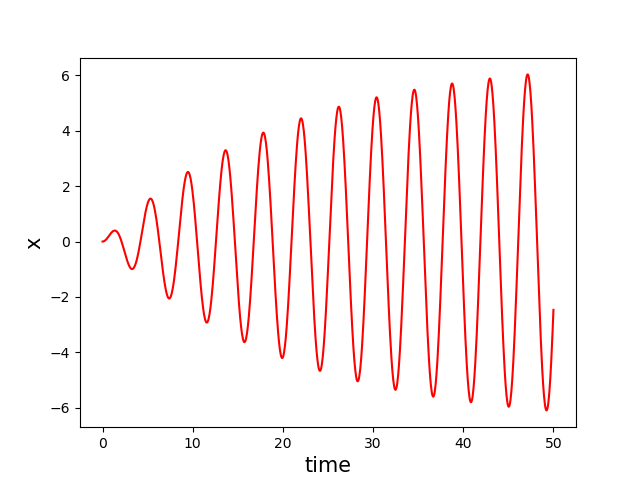
\includegraphics[scale=0.6]{fig1.png}
\caption{System Response with Decay = 0.5}
\label{fig:System Response with Decay = 0.05}
\end{figure}

\clearpage
\subsection{Response over different frequencies}
Model the system as an LTI system,the following graphs are obtained
by varying the frequency of the force $f(t)$.
\begin{figure}[h!]
\centering
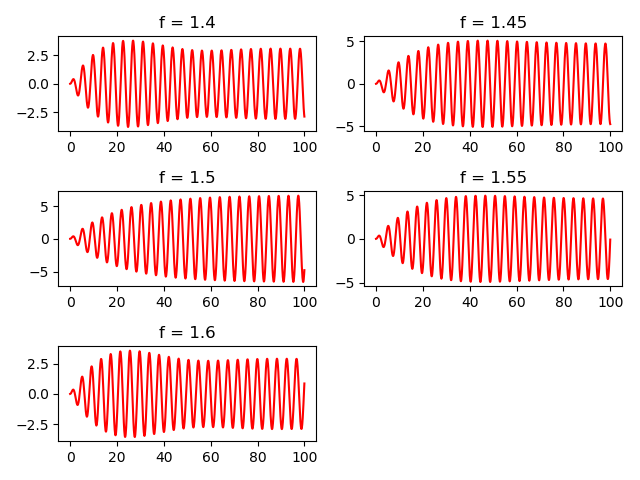
\includegraphics[]{fig2.png}
\caption{System Response with frequencies from 1.4 to 1.6}
\label{fig:System Response with frequencies from 1.4 to 1.6}
\end{figure}
From the given equation, we can see that the natural response of the system has the frequency w = 1.5 rad/s . Thus, as expected the maximum amplitude of oscillation is obtained when the frequency of $f(t)$ is 1.5 rad/s, due to resonance.
\clearpage


\subsection{The coupled spring problem}

We now consider a coupled Differential system
\begin{equation}
    \ddot x + (x-y) = 0
\end{equation}
and 
\begin{equation}
    \ddot y + 2(y-x) = 0
\end{equation}

with the initial conditions: $\dot x(0) =0,\dot y(0) =0,x(0) =1,y(0) =0$.
Taking Laplace Transform and solving for $X(s)$ and $Y(s)$, We get:
\begin{equation}
    X(s) = \frac{s^2+2}{s^3 + 3s}
\end{equation}
\begin{equation}
    Y(s) = \frac{2}{s^3 + 3s}
\end{equation}

We notice that the outputs of this system are 2 sinusoids which are out of phase. This system can be realized by creating an undamped single spring double mass system.
\begin{figure}[h!]
\centering
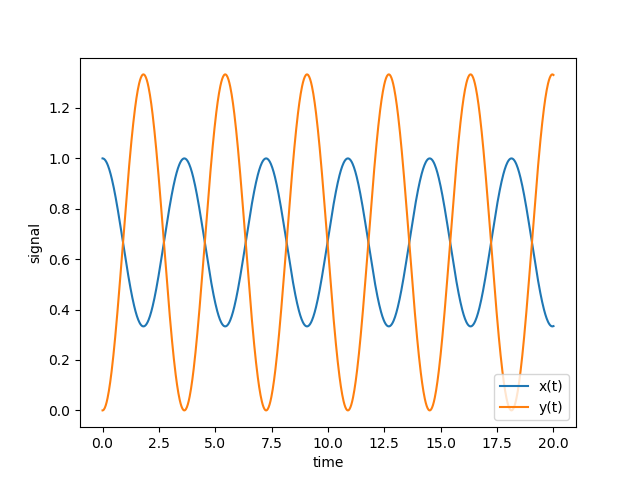
\includegraphics[scale=0.6]{fig3.png}
\caption{Coupled Oscillations}
\label{fig:Coupled Oscillations}
\end{figure}
\clearpage


\subsection{The Two-Port Network}
The Steady-State transfer function of the given circuit is given by

\begin{equation}
    H(s) = \frac{10^6}{s^2 + 100s + 10^6}
\end{equation}

The magnitude and phase response are as follows:


\begin{figure}[h!]
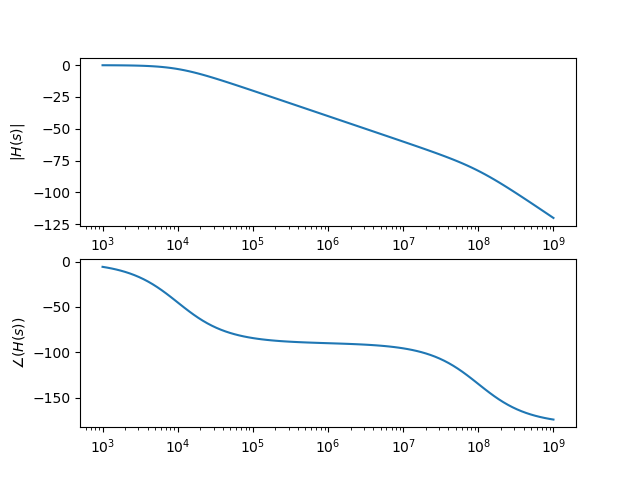
\includegraphics[scale=0.8]{fig4.png}
\centering
\caption{Bode Plots For RLC Low pass filter}
\label{fig:Coupled Oscillations}
\end{figure}

Plot the response of the low pass filter to the input:\newline
\begin{center}
$V_i(t) = (cos(10^3t) - cos(10^6t))u(t)$
\end{center}
for $0<t<30\mu s$ and $0<t<30ms$



\begin{figure}[h!]
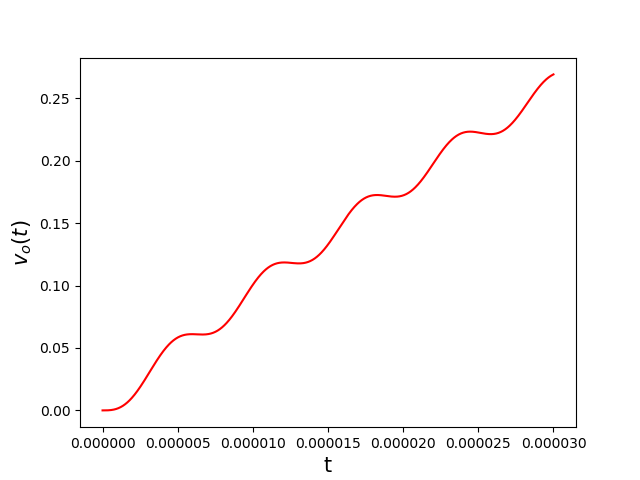
\includegraphics[scale=0.6]{fig5.png}
\centering
\caption{System response for t $<$ 30us}
\label{fig:Coupled Oscillations}
\end{figure}
\begin{figure}[h!]
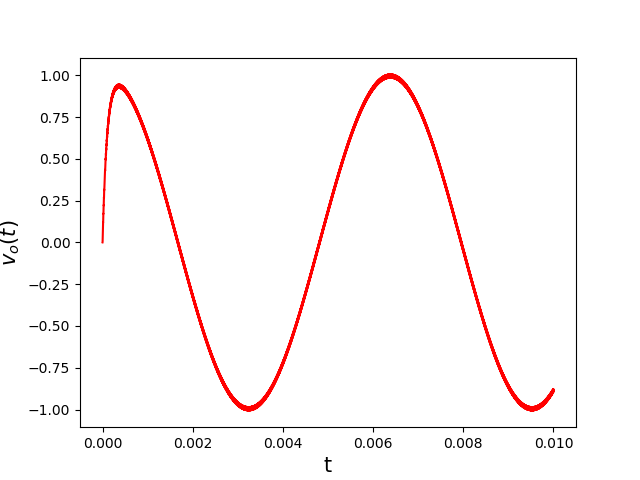
\includegraphics[scale=0.6]{fig6.png}
\centering
\caption{System response for t $<$ 10ms}
\label{fig:Coupled Oscillations}
\end{figure}

From the Bode plot of $H(s)$ we can see that the system acts like a low pass filter. It provides unity gain for frequency less than $10^3$ rad/s. Thus the low frequency component remains same. On the other hand, the system dampens the high frequency component with $|H(s)|_{dB}$ approximately 0.
\clearpage

\section{Conclusion}
The scipy.signal library provides a useful toolkit of functions for circuit analysis. The toolkit was used for the analysis of LTI systems in various domains.\\
The forced response of a simple spring body system was obtained over various frequencies of the applied force, and highest amplitude was observed at resonant frequency.\\
A coupled spring problem was solved using the sp.impulse function to obtain two sinusoids of the same frequency.\\
A two-port network, functioning as a low-pass filter was analysed and the output was obtained for a mixed frequency input.
\end{document}
